\documentclass[10.5pt]{article}
\usepackage[utf8]{inputenc}
\usepackage{graphicx}
\usepackage[margin = 0.70in]{geometry}
\usepackage{pdfpages}
\usepackage{listings}
\usepackage{xcolor}
\usepackage{array}
\usepackage{appendix}
\usepackage{sectsty}
\usepackage{hyperref}
\usepackage{float}
\usepackage{wrapfig}
\usepackage{subfig}

\definecolor{codegreen}{rgb}{0,0.6,0}
\definecolor{codegray}{rgb}{0.5,0.5,0.5}
\definecolor{codepurple}{rgb}{0.58,0,0.82}
\definecolor{backcolour}{rgb}{0.95,0.95,0.92}

\lstdefinestyle{mystyle}{
    commentstyle=\color{codegreen},
    keywordstyle=\color{blue},
    numberstyle=\tiny\color{codegray},
    stringstyle=\color{codepurple},
    basicstyle=\ttfamily\footnotesize,
    breakatwhitespace=false,         
    breaklines=true,                 
    captionpos=b,                    
    keepspaces=true,                 
    numbers=left,                    
    numbersep=5pt,                  
    showspaces=false,                
    showstringspaces=false,
    showtabs=false,                  
    tabsize=2
}

\lstset{style=mystyle}
\sectionfont{\bfseries\Large\raggedright}
\renewcommand{\thesubsection}{\thesection.\alph{subsection}}
\begin{document}
\pagenumbering{arabic}
%begin{titlepage}
    
\begin{center}
    \vspace*{-2cm}+
    %\textsc{\large DEPARTMENT OF ELECTRONIC AND TELECOMMUNICATION ENGINEERING
    %\\ [2mm]
    %UNIVERSITY OF MORATUWA}\\
    %[0.5cm]

    \textsc{\large EN2550 FUNDAMENTALS OF IMAGE PROCESSING AND MACHINE VISION}\\
    [3mm]
    \line(1,0){300}\\
    [1mm]
    \huge{\bfseries  ASSIGNMENT 02 - Fitting and Alignment} \\
    \line(3,0){300}\\
[0.3cm]  
\end{center}
\begin{center}
    Thanushan K.
    \hspace*{1cm}
    190621M
\end{center}
\vspace*{0.25cm}
%\begin{center}
%    This is submitted as a partial fulfilment for the module EN2550.\\
%    \line(10,0){50}\\
%    [0.25cm]
%    \today
%\end{center}
%\end{titlepage}


\begin{flushleft}
\section{RANSAC Implementation}
RANSAC is a general framework used for fitting models when there are outliers present in the matching features found in the images used to stitch. In this question, we have to fit a circle using the RANSAC algorithm for a randomly generated set of points. 
The probability that atleast one sample is free from outliers (p) is set to be 0.99. The outlier ratio (e) was set to 0.5, considering the worst case. The threshold of selecting inliers was set to 1. The number of samples N was calculated using equation 1.
\begin{equation}\label{Equation 1: Number of samples}
    N = \frac{\log(1-p)}{\log(1-(1-e)^{min_s})}
\end{equation}
Three random samples were selected in each iteration, because we need atleast 3 points ($min_{s}$) to find the equation of the circle. The circle was found corresponding to the sample points. The inliers are found using the threshold. The current set of inliers is compared with the set of inliers obtained from the previous sample and the set with maximum number of inliers is selected. The iteration goes upto N iterations. Then the RANSAC algorithm is run by giving the final set of inliers obtained as the input inorder to obtain the best fit circle. 
\newline
When considering the results, the best fit circle and the circle drawn using the sample points, which give the set with maximum inliers, are almost similar to each other. The code and Output are shown in figures 1 and 2 respectively.    

\begin{figure}[htp]
    \centering
    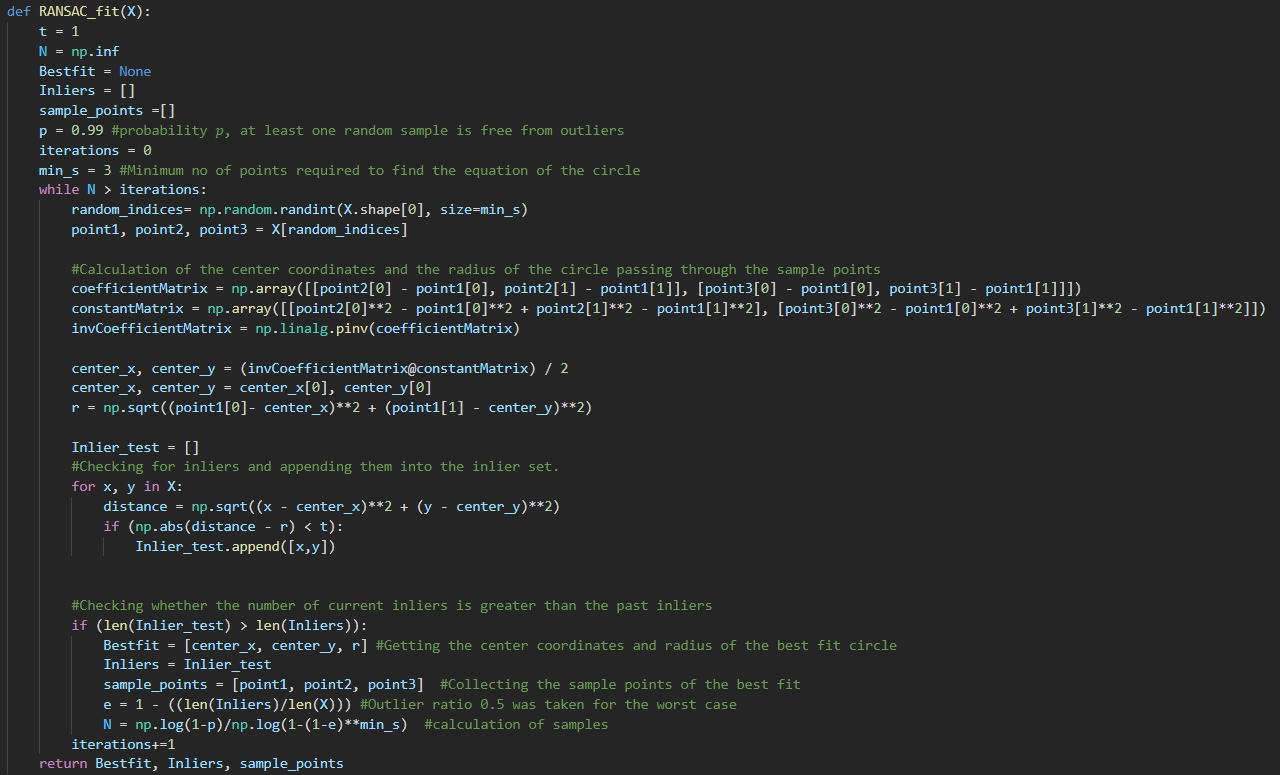
\includegraphics[width=0.8\textwidth]{Question1code.png}
    \caption{Code for RANSAC Algorithm}
\end{figure}

\begin{figure}[htp]
    \centering
    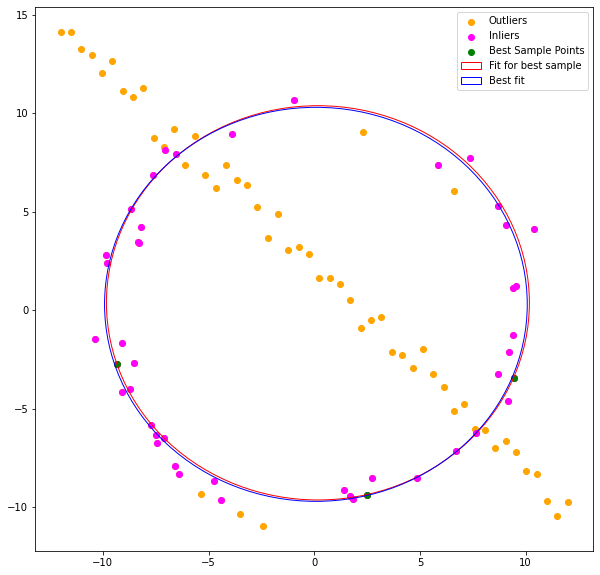
\includegraphics[width=0.4\textwidth]{Question1output.png}
    \caption{RANSAC Circle Fitting}
\end{figure}

\begin{figure}
    \subfloat[mousePoints function]{{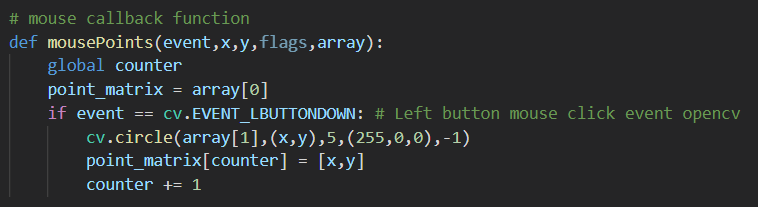
\includegraphics[width=8.0cm]{Question2code1.png}}}
    \qquad
    \subfloat[Loop for selecting points]{{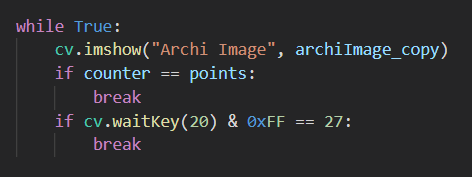
\includegraphics[width=7.0cm]{Question2code2.png}}}
    \caption{Mouse click algorithm}
    \label{fig:example}
\end{figure}
\section{Image Warping and Blending by calculating a hormography}
In this question, we have to warp and blend one image to another. Initially we have to select 4 points (We get four points because it is the minimum number of points required to calculate the homography matrix) in the background image. This can be done by the setMouseCallback function in the opencv library. After getting the four coordinate points of the background image and the four corner coordinates of the image to be warped, we create a matrix A which is the coeffiecient matrix of the homography vector. We calculate the eigenvalues and eigenvectors using equation 2. The eigen vector corresponding to the minimum eigen value is taken and constructed into a $3X3$ matrix to get the homography matrix. Then the image is warped according to the corresponding homography matrix and added to the background image.
Two other pairs of images were chosen and the algorithm was tested. The essential codes are shown in figures 3 and 4. The results are shown in figure 5.
\begin{equation}\label{Equation 2: hormography equation}
     A.H = 0
\end{equation}

\begin{figure}[htp]
    \centering
    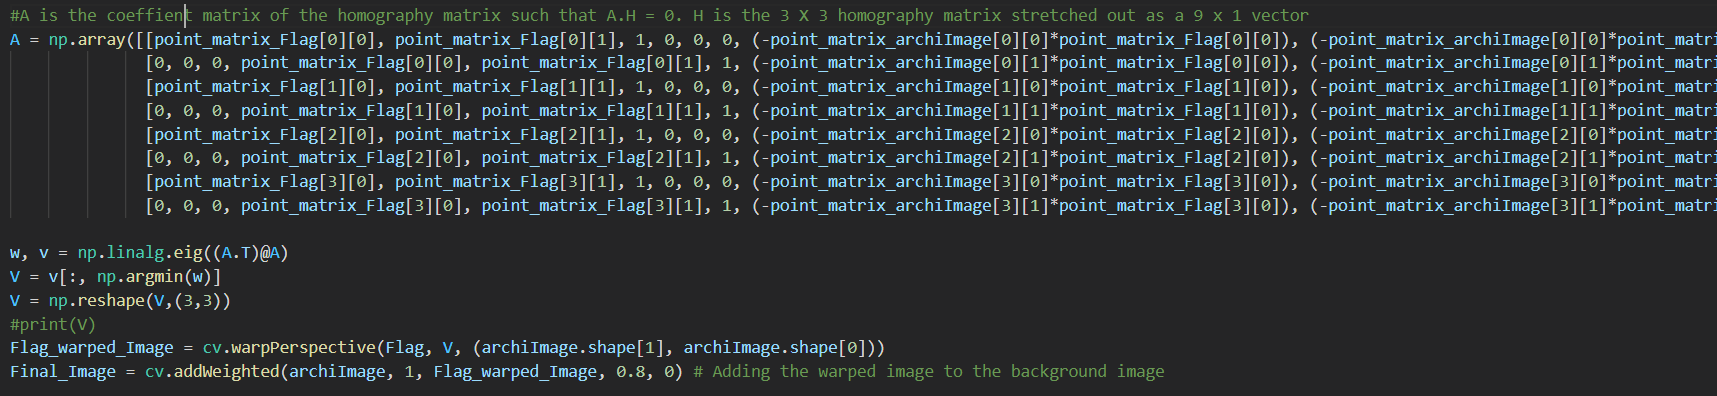
\includegraphics[width=0.6\textwidth]{Question2code3.png}
    \caption{Homography calculation}
\end{figure}

\begin{figure}
    \centering
    \subfloat[Output 1]{{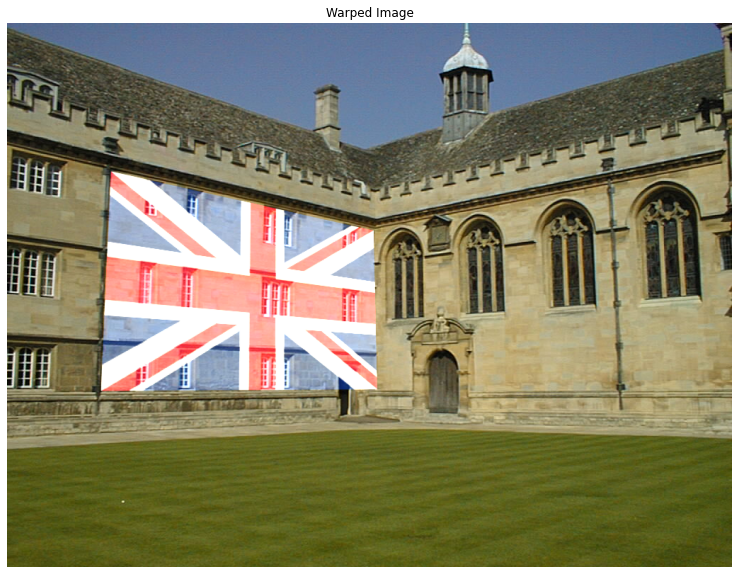
\includegraphics[width=4.0cm]{Question2output21png.png}}}
    \qquad
    \subfloat[Output 2]{{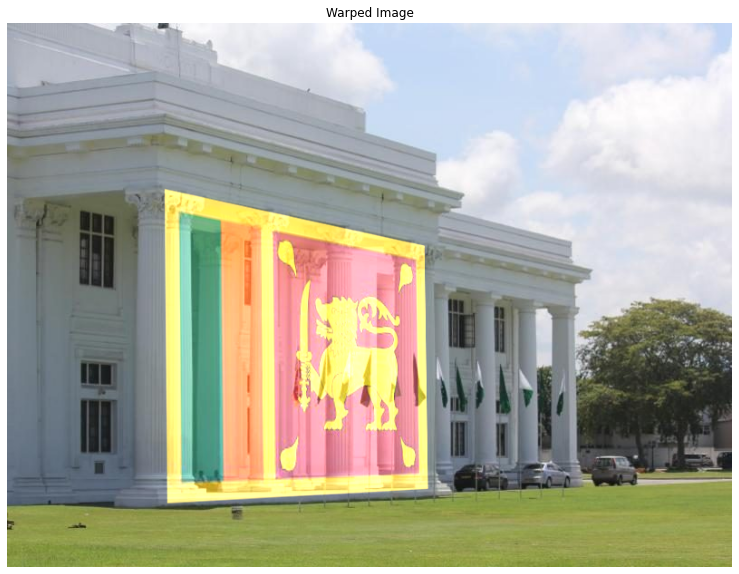
\includegraphics[width=4.0cm]{Question2output2.png}}}
    \qquad
    \subfloat[Output 3]{{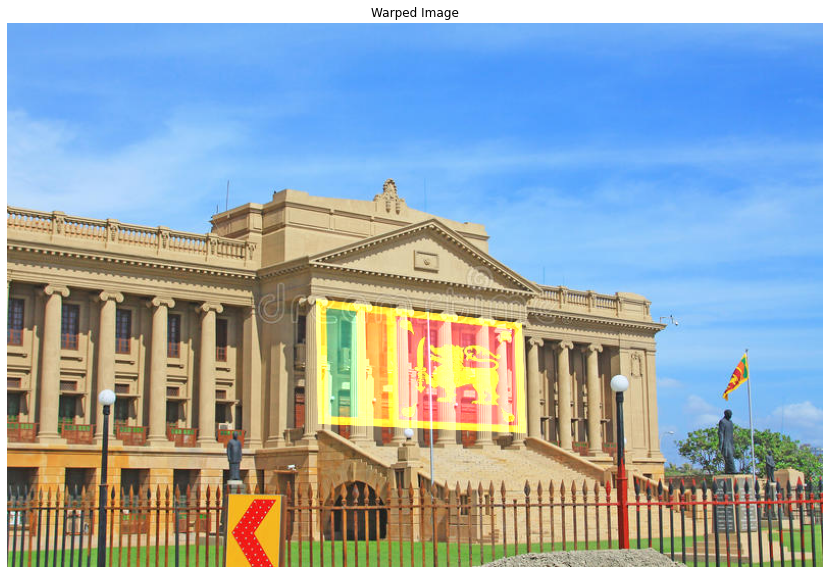
\includegraphics[width=4.0cm]{Question2output3.png}}}
    \caption{Outputs for Warping and blending}
    \label{fig:example2}
\end{figure}

\section{Stitching Two Images by computing a hormography using RANSAC }
In this problem we have to stitch two images by calculating the homography matrix by identifying the matching points between the 2 images using the SIFT algorithm.
\subsection{SIFT Feature extraction}
In this section, we have to find the SIFT features between image 1 and image 5 in the grafitti image sequence. Flann based matcher is used to identify the matching features between the images. The output is shown in figure 6.a. and the relevant code is shown in figure 6.b.
\begin{figure}
    \centering
    \subfloat[Output]{{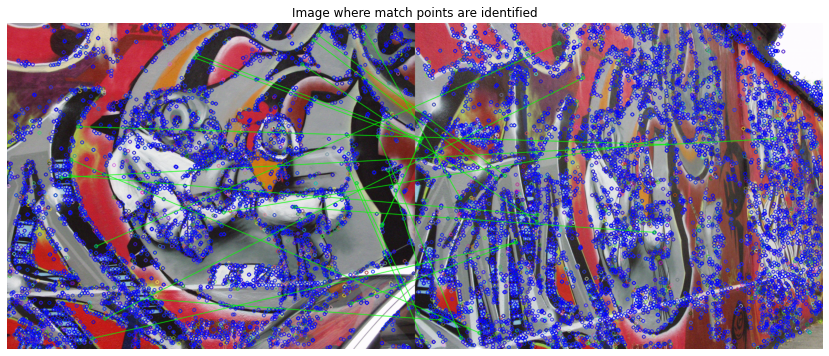
\includegraphics[width=8.0cm]{Question3SIFT.png}}}
    \qquad
    \subfloat[Code]{{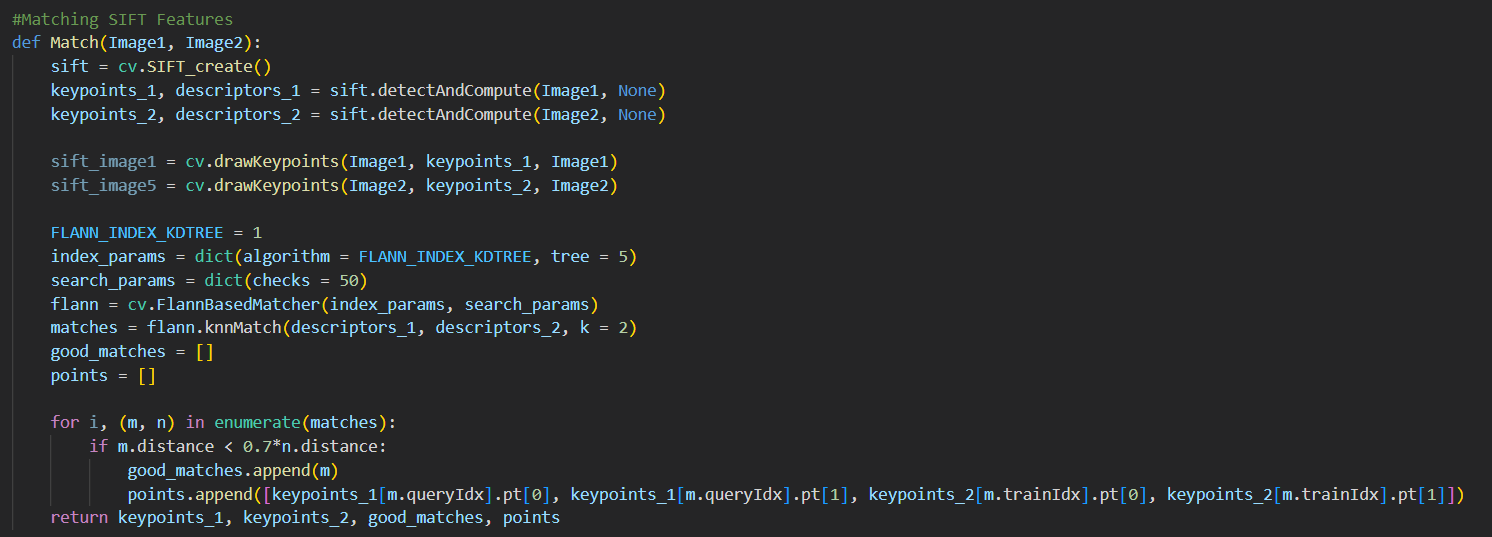
\includegraphics[width=9.0cm]{Question3code3.png}}}
    \caption{SIFT Feature Extraction}
    \label{fig:example}
\end{figure}

\subsection{Homography calculation}
In this section, we have to calculate the homography matrix that transforms image 1 to image 5. The best homography matrix is identified using the RANSAC algorithm. Four random points are selected from the good matches found from the SIFT feature extraction. Then a homography matrix is calculated by using the selected four points using equation 3. The homography is calculated by finding the eigenvector corresponding to the minimum eigenvalue of the matrix $A^{T}A$ and reshaping it to a $3 X 3$ matrix.
Then, the destination point is calculated to each and every point in the matchpoints set using the homography matrix. The difference between the calculated value and the actual value is calculated. If the difference is less than a certain threshold, the point set is added to the currentt inlier set. The homography matrix that gives the maximum number of inliers is selected as the final answer. The calculated homography matrix is compared with the given homography matrix. 
The homography between image 1 and image 5 could not be achieved accurately because the number of good match points found using SIFT was not sufficient. Therefore, the homographies between images 1 and 2, 2 and 3, 3 and 4, and 4 and 5 were found. Then the product of these homography matrices were calculated to find the final result. The calculated final homography values were very much close to the given homography values. Relevant codes are shown in figure 7.
\begin{equation}\label{Equation 3: hormography equation}
    A.H = 0
\end{equation}
\begin{figure}
    \centering
    \subfloat[Code]{{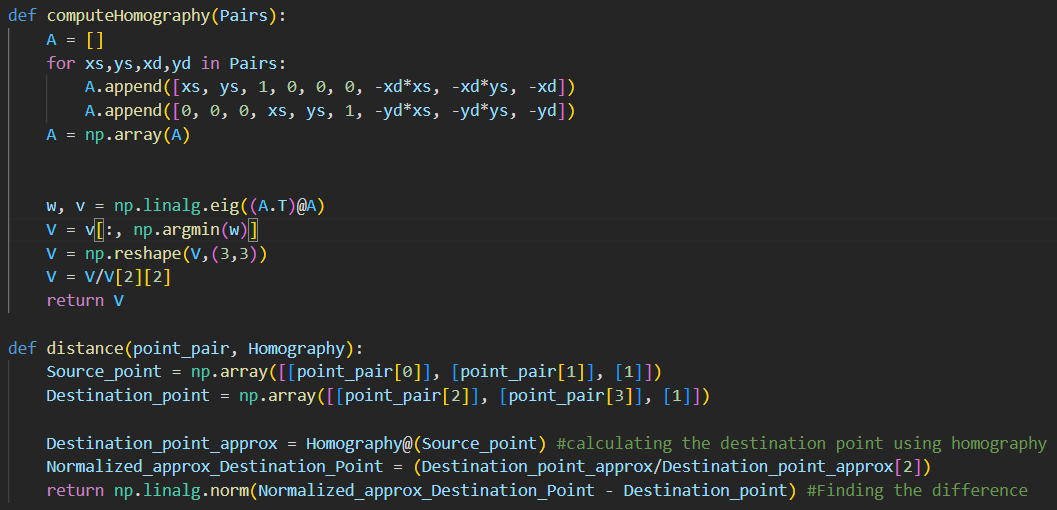
\includegraphics[width=8.0cm]{Question3code1.png}}}
    \qquad
    \subfloat[Code]{{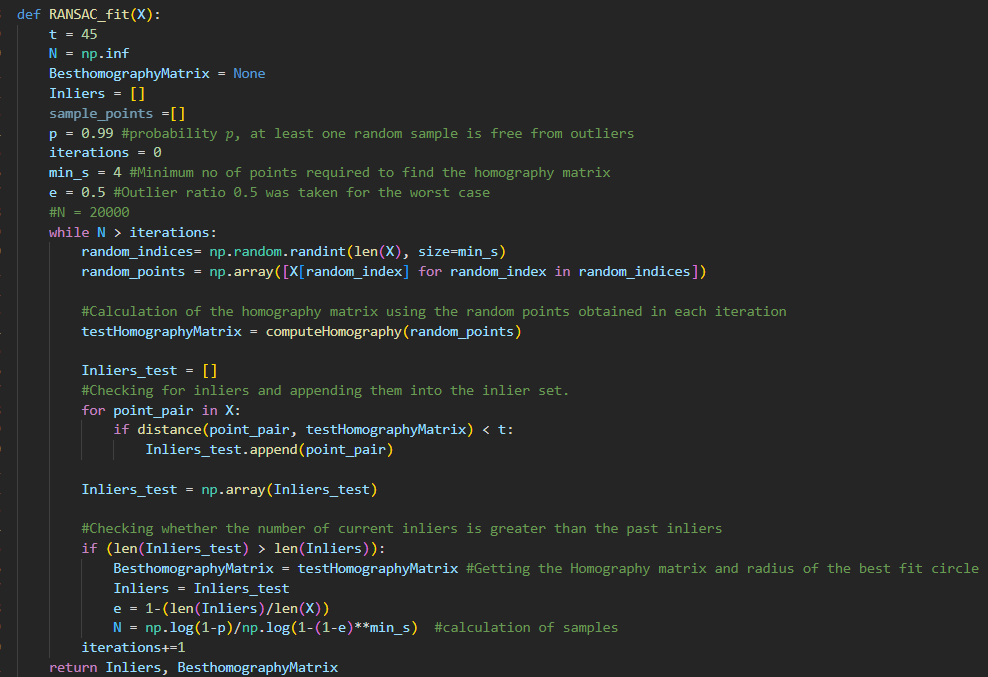
\includegraphics[width=9.0cm]{Question3code2.png}}}
    \caption{Homography calculation}
    \label{fig:example}
\end{figure}



\subsection{Stitching Images}
\begin{figure}[htp]
    \centering
    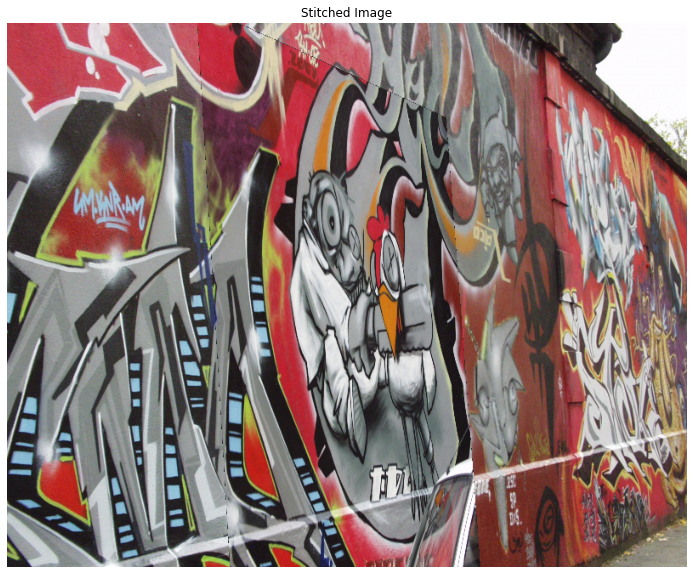
\includegraphics[width=0.3\textwidth]{Question3Stitched.png}
    \caption{Final stitched image}
\end{figure}
In this section, we have to stitch the images according to the homography matrix calculated in the above section. Image 1 is warped to the alignment of image 5 using the warpPerspective function in the opencv library. The background image is cut using the warped image as a mask. Then the images are stitched by using the addWeighted function in opencv.
The output is shown in figure 8.
\\
\textbf{Code Files} : All relevant codes and files can be found in \href{https://github.com/K-Thanushan/EN2550-Fundamentals-of-Image-Processing-and-Machine-Vision/tree/main/Assignments/Assignment1}{\textbf{\underline{GitHub}}}.

\end{flushleft}

\end{document}